\documentclass[conference]{IEEEtran}
\usepackage[utf8]{inputenc}
\usepackage[T1]{fontenc}
\usepackage{graphicx,booktabs,url,hyperref,xcolor,listings,amsmath,array}
\usepackage{tikz}
\usetikzlibrary{arrows.meta,positioning,shapes.geometric,fit,calc}
\hypersetup{colorlinks,linkcolor=black,citecolor=blue,urlcolor=blue}
\newcommand{\ffrs}{FFRS}
\newcommand{\todo}[1]{\textcolor{red}{[TODO: #1]}}
% Draft banner: set \draftnote to empty for the submitted version.
\newcommand{\draftnote}{Work-in-progress draft, 19 August 2026 --- not peer reviewed; evaluation section pending the week-4 read-out (15 September 2026). Comments welcome.}
\lstset{basicstyle=\ttfamily\footnotesize,breaklines=true,frame=single}

\title{Fast Feedback Resolution System (FFRS): A Five-Stage Pipeline from Capture to Close with an Agentic Respond Stage}

\author{\IEEEauthorblockN{Ganesh Butcha}
\IEEEauthorblockA{ScaledAIOps \\ ganesh35@gmail.com}
\thanks{\draftnote}}

\begin{document}
\maketitle

\begin{abstract}
Small software projects rarely close the loop with the people who report bugs or request features. Capture is easy; what follows---acknowledgement, a first substantive response, a decision, and notice of the outcome---is unowned, unmeasured, and therefore slow. This paper presents the Fast Feedback Resolution System (\ffrs), a model that runs each feedback item through a five-stage pipeline (capture, acknowledge, route, respond, close) in which every stage is a timestamp recorded by the system that owns it. Its defining element is an \emph{agentic Respond stage}: a scheduled AI agent produces the first substantive response to every item---for changes it can make, a complete pull request with tests and evidence for a developer to review and merge; otherwise a proposal that is executed only after the requester accepts it and a reviewer confirms it. No agent action takes effect without a human decision. Because the stages are timestamps, the metrics follow without manual bookkeeping. We describe a dependency-minimal, tool-agnostic reference architecture---a 5\,KB (gzipped) widget, one serverless function, the project's existing issue tracker as system of record, a private sidecar for the only personal datum, and a scheduled coding agent---and its open implementation, run as one shared, multi-tenant service and evaluated on two sites from 23~September~2026: the project's reference site, whose Respond stage is agentic, and an anonymous B2B quick-commerce platform that responds manually through the same pipeline. We report \todo{$n$} items over \todo{$k$} weeks (median time to first response \todo{$x$}, loop closure \todo{$y$}\%, agent share \todo{$z$}\%) against pre-registered targets and characterise when a minimal, human-reviewed agentic loop is sufficient. All artefacts are open; the reference site's metrics are recomputable from public data.
\end{abstract}

\begin{IEEEkeywords}
user feedback, feedback loops, AI agents, human-in-the-loop, issue tracking, DevOps metrics, software maintenance
\end{IEEEkeywords}

\section{Introduction}
Every software project has a channel through which stakeholders raise feature requests (FRs) and bug reports (BRs). Far fewer have a working \emph{loop}: an item that is registered, acknowledged, acted upon, and whose outcome is reported back to the person who raised it. In the author's experience across two decades of projects, the failure is seldom at capture---forms, mail, tickets and trackers abound---but in the interval that follows. Items wait for a triage meeting, for a developer with capacity, for a decision; the requester hears nothing; and because that interval is unmeasured, its cost is invisible.

Two things have changed. First, the tooling that small teams already use---a Git host with an issue tracker, a serverless function, a mail API---is enough to record every stage of a feedback item as a timestamp, which makes response behaviour measurable for free. Second, AI coding agents can now read an issue, change code, run tests and open a pull request unattended. This makes it realistic to \emph{assign the Respond stage to an agent by default} and to reserve human effort for review, acceptance and merge.

The Fast Feedback Resolution System (\ffrs) is the author's synthesis of these two observations into a small, prescriptive model: a pipeline with five stages---capture, acknowledge, route, respond, close---four timestamp-derived metrics, and one structural rule: the Respond stage is performed by a scheduled agent, with two paths. For items that require a code change, the agent produces a complete pull request---the fix, the tests it ran, and the evidence---for a developer to review and merge. For items that do not, the agent proposes a solution; the proposal is executed only after the \emph{requester} accepts it and a \emph{reviewer} confirms it. The loop closes when the outcome is recorded and reported back.

\subsection{Contributions}
\begin{enumerate}
  \item \textbf{The \ffrs{} model} (Sec.~\ref{sec:model}): stages, the two-path agentic Respond stage with its human checkpoints, and metrics defined purely from timestamps.
  \item \textbf{A tool-agnostic reference architecture} (Sec.~\ref{sec:arch}) defined by roles and contracts---tracker, function, object store, mail, bot check, coding agent---in which the project's existing issue tracker serves as the system of record, so that anyone with read access can recompute all metrics and each role can be filled by any equivalent product.
  \item \textbf{An open implementation} (Sec.~\ref{sec:impl}): a 4\,KB widget, one serverless function, and a scheduled agent, live on scaledaiops.org.
  \item \textbf{An evaluation} (Sec.~\ref{sec:eval}) on two sites against a pre-registered protocol, and an analysis of which parts of the design are load-bearing.
\end{enumerate}

\subsection{Research questions}
\begin{itemize}
  \item \textbf{RQ1} Can the \ffrs{} model, including the agentic Respond stage, be implemented for a small project with no database and no third-party feedback vendor, and what does it cost to build and run?
  \item \textbf{RQ2} What response and closure behaviour does it produce in practice---time to first response, time to close, loop closure, signal ratio, and the share of items resolved by an agent-authored pull request?
  \item \textbf{RQ3} Which parts of the design are load-bearing for those outcomes, and which could be removed?
\end{itemize}

\section{Background and Motivation}
\subsection{The interval nobody owns}
Consider the reference site of this paper, scaledaiops.org: a static, volunteer-maintained reference for an AI-operations framework, without accounts or analytics. Until August 2026 its only feedback path was a link to the project's code-hosting organisation. A visitor without an account there could not report anything; one with an account had to leave the site, choose a repository and open an issue; nobody was notified; and no one could say how long such an issue typically waited. This is not unusual. Service desks and DevOps teams solve the same problem with people and process---ITIL-style acknowledgement, routing and resolution targets~\cite{axelos2019itil}, or flow metrics such as lead time and time to restore~\cite{forsgren2018accelerate}---but those presume staff whose job it is to work the queue.

\subsection{What ``small'' means here}
We use \emph{small project} operationally: at most three maintainers, no dedicated support or triage role, and fewer than one hundred feedback items per month. At that scale a vendor feedback product is disproportionate (data leaves the project, cost per seat, another login), a self-hosted tracker is another system to operate, and the raw Git host is unfriendly to outsiders. \ffrs{} targets exactly this gap.

\subsection{Why an agent changes the economics}
The scarce resource in a small project is maintainer attention. If the first substantive response to an item---a candidate fix with tests, or a concrete proposal---can be produced without it, attention is spent only on judgement: is the fix right, is the proposal acceptable. An independent commercial site that implemented a comparable capture widget (with a conventional, manual response process) reports the same pattern: capture works, items still stall. That observation motivated making the agentic stage a defining part of the model rather than an optional add-on.
The author's own path---systems administration in the 2000s, web development in the 2010s, then DevOps and release management for large delivery organisations---crossed the same failure repeatedly: feedback was captured diligently and acted on late or never, and nobody could say how late. What was missing was never a form; it was an owner for the interval after the form, and a clock on it. \ffrs{} is that owner and that clock, with the owner now an agent.

\section{The \ffrs{} Model}\label{sec:model}
\subsection{Stages}
The \ffrs{} model treats feedback as a five-stage pipeline (Fig.~\ref{fig:pipeline}). Each stage is a single timestamp, recorded by the system that naturally owns the event (Table~\ref{tab:stages}); \ffrs{} prescribes no additional bookkeeping.

\begin{figure}[h]
\centering
\resizebox{\columnwidth}{!}{%
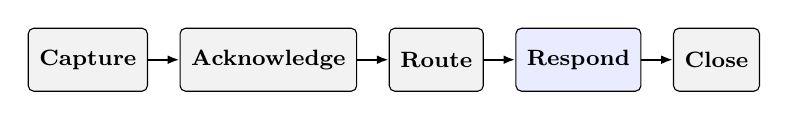
\begin{tikzpicture}[
  font=\footnotesize, node distance=4mm,
  stage/.style={draw, rectangle, rounded corners=2pt, inner sep=4pt, align=center, minimum height=8mm, fill=black!5},
  arr/.style={-{Latex[length=1.5mm]}, thick}
]
  \node[stage] (cap) {\textbf{Capture}};
  \node[stage, right=of cap] (ack) {\textbf{Acknowledge}};
  \node[stage, right=of ack] (rte) {\textbf{Route}};
  \node[stage, right=of rte, fill=blue!8] (rsp) {\textbf{Respond}};
  \node[stage, right=of rsp] (cls) {\textbf{Close}};
  
  \draw[arr] (cap) -- (ack);
  \draw[arr] (ack) -- (rte);
  \draw[arr] (rte) -- (rsp);
  \draw[arr] (rsp) -- (cls);
\end{tikzpicture}%
}
\vspace{-2mm}
\caption{The five-stage \ffrs{} pipeline. The \emph{Respond} stage is agentic by default.}
\label{fig:pipeline}
\end{figure}

\begin{table}[t]
\centering\footnotesize
\caption{\ffrs{} stages. ``Owner'' is the system whose clock records the timestamp.}
\label{tab:stages}
\begin{tabular}{@{}l>{\raggedright\arraybackslash}p{3.6cm}>{\raggedright\arraybackslash}p{2.6cm}@{}}
\toprule
Stage & Definition & Owner / timestamp \\
\midrule
Capture & The item exists durably with a public reference id & tracker: issue created \\
Acknowledge & Requester is told it was received (only if they asked to be) & mail: ack sent \\
Route & Item is in the working tool with kind/severity labels & tracker (may equal Capture) \\
Respond & First substantive response: an agent PR or proposal, or a human comment & tracker: first comment / PR \\
Close & Outcome recorded and reported to the requester & tracker: closed; mail: closing note \\
\bottomrule
\end{tabular}
\end{table}

\subsection{The agentic Respond stage}
Respond is performed by a scheduled agent that reads every open item not yet responded to. It follows one of two paths (Fig.~\ref{fig:paths}):

\paragraph{Code path} If the item implies a code or content change the agent can make, it produces a \emph{complete pull request}: the change, the tests it wrote or ran, their results, and a link back to the item. A developer reviews and merges (or rejects with a reason). Merge closes the item with outcome \emph{fixed} or \emph{shipped}.

\paragraph{Proposal path} Otherwise the agent posts a \emph{proposal}: what it would do, what it needs, and any risk. Two human checkpoints follow: the \emph{requester} accepts (the proposal solves their problem) and a \emph{reviewer} confirms (it is safe and appropriate for the project). Only then does the agent execute and close the item; a rejection at either checkpoint returns it to the human queue. If the requester does not respond within a staleness timeout (e.g., 14 days), the item is automatically closed to prevent unbounded queue growth.

The rule that makes \ffrs{} ``fast'' is that the first substantive response is produced without waiting for a maintainer, and that maintainer effort is spent on judgement rather than production. The rule that keeps it safe is that nothing the agent produces takes effect without a human decision: merge, or accept-and-confirm.

\begin{figure}[t]
\centering
\resizebox{\columnwidth}{!}{%
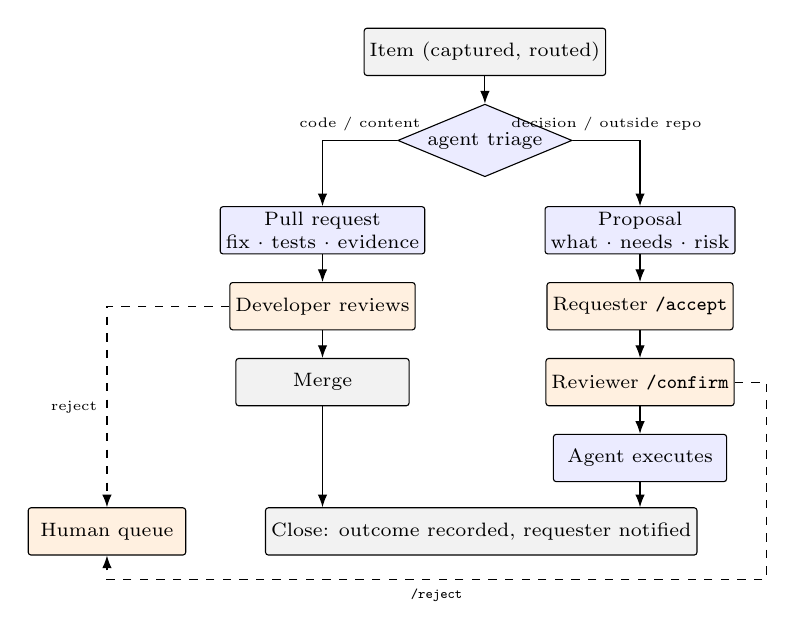
\begin{tikzpicture}[
  font=\scriptsize, node distance=3.5mm and 6mm,
  box/.style={draw, rounded corners=1pt, minimum height=6mm, minimum width=22mm, inner sep=2pt, align=center},
  agent/.style={box, fill=blue!8}, human/.style={box, fill=orange!12}, sys/.style={box, fill=black!5},
  dec/.style={diamond, draw, aspect=2.4, inner sep=1pt, align=center, fill=blue!8},
  arr/.style={-{Latex[length=1.6mm]}}, rej/.style={arr, dashed}]
  \node[sys] (item) {Item (captured, routed)};
  \node[dec, below=of item] (tri) {agent triage};
  \node[agent, below left=6mm and 2mm of tri] (pr) {Pull request\\fix $\cdot$ tests $\cdot$ evidence};
  \node[human, below=of pr] (rev) {Developer reviews};
  \node[sys, below=of rev] (merge) {Merge};
  \node[agent, below right=6mm and 2mm of tri] (prop) {Proposal\\what $\cdot$ needs $\cdot$ risk};
  \node[human, below=of prop] (acc) {Requester \texttt{/accept}};
  \node[human, below=of acc] (conf) {Reviewer \texttt{/confirm}};
  \node[agent, below=of conf] (exec) {Agent executes};
  \node[sys, below=8mm of $(merge.south)!0.5!(exec.south)$] (close) {Close: outcome recorded, requester notified};
  \node[human, left=10mm of close, minimum width=20mm] (queue) {Human queue};
  \draw[arr] (item) -- (tri);
  \draw[arr] (tri) -| node[pos=0.25, above, font=\tiny]{code / content} (pr);
  \draw[arr] (tri) -| node[pos=0.25, above, font=\tiny]{decision / outside repo} (prop);
  \draw[arr] (pr) -- (rev); \draw[arr] (rev) -- (merge);
  \draw[arr] (prop) -- (acc); \draw[arr] (acc) -- (conf); \draw[arr] (conf) -- (exec);
  \draw[arr] (merge) -- (close.north -| merge); \draw[arr] (exec) -- (close.north -| exec);
  \draw[rej] (rev.west) -| node[pos=0.75, left, font=\tiny]{reject} (queue.north);
  \draw[rej] (conf.east) -- ++(4mm,0) |- ($(queue.south)+(0,-3mm)$) node[pos=0.75, below, font=\tiny]{\texttt{/reject}} -- (queue.south);
\end{tikzpicture}}
\caption{The agentic Respond stage. Blue: produced by the agent; orange: human decisions; grey: system events. Nothing the agent produces takes effect without a merge or an accept-and-confirm.}
\label{fig:paths}
\end{figure}

\subsection{Metrics Formalization}
Let $\mathcal{I}$ be the set of feedback items in a given reporting window, partitioned by kind. For each item $i \in \mathcal{I}$, the pipeline records a tuple of monotonically increasing timestamps $\langle t_{\text{cap}}(i), t_{\text{ack}}(i), t_{\text{route}}(i), t_{\text{resp}}(i), t_{\text{close}}(i) \rangle$. For agent-driven systems, we additionally record $t_{\text{human}}(i)$, the timestamp of the first human decision.

All duration metrics are derived directly from these timestamps:
\begin{align}
  \text{TTFR}(i) &= t_{\text{resp}}(i) - t_{\text{cap}}(i) \\
  \text{TTHR}(i) &= t_{\text{human}}(i) - t_{\text{cap}}(i) \\
  \text{TTC}(i) &= t_{\text{close}}(i) - t_{\text{cap}}(i)
\end{align}
Aggregates are reported as p50 and p90. Systemic rates are defined as follows, where $\mathcal{I}_{\text{closed}}$ is the subset of items that reached the Close stage:
\begin{align}
  \text{Loop Closure} &= \frac{|\mathcal{I}_{\text{closed}}|}{|\mathcal{I}|} \\
  \text{Signal Ratio} &= 1 - \frac{|\mathcal{I}_{\text{spam}} \cup \mathcal{I}_{\text{dup}}|}{|\mathcal{I}|} \\
  \text{Agent Share} &= \frac{|\mathcal{I}_{\text{agent\_merged}} \cup \mathcal{I}_{\text{agent\_exec}}|}{|\mathcal{I}_{\text{closed}}|}
\end{align}
For items whose requesters opted in, we track the \emph{consented notification rate} as the share for which the closing note was successfully sent. These definitions are deliberate analogues of flow metrics~\cite{forsgren2018accelerate} and service-desk targets~\cite{axelos2019itil}, reduced to what the system's timeline can witness.

\subsection{Design principles}
\begin{enumerate}
  \item \emph{Durable first.} The item exists in the tracker before any notification or agent action.
  \item \emph{Automate everything but judgement.} Ack, route, first response and closing notification are code; merge, accept and confirm are people.
  \item \emph{Measure timestamps, not opinions.} No status field is hand-maintained; metrics are recomputable by anyone with read access to the tracker.
  \item \emph{Responsible by default.} Personal data only with consent, stored apart from the public record, deletable; the agent never acts on production without a human checkpoint.
  \item \emph{Everything through version control.} Infrastructure as code and GitOps for every layer---site content, widget, function, cloud resources, the agent's own instructions---so that each change, human or agent, is a reviewed commit and the audit trail is the commit log.
\end{enumerate}

\section{Reference Architecture}\label{sec:arch}
Fig.~\ref{fig:arch} shows the reference architecture in terms of \emph{roles}; Table~\ref{tab:roles} lists, for each role, the component used in the reference deployment and equivalent alternatives. \ffrs{} prescribes the roles and the contracts between them, not the products: any tracker with issues, comments, labels and webhooks; any function-as-a-service runtime; any object store; any transactional mail API; any bot check; any coding agent that can open a pull request. The guiding constraint was that a small project should add \emph{no} new system of record: the issue tracker it already uses \emph{is} the store.

\begin{table}[t]
\centering\footnotesize
\caption{Roles in the reference architecture, the component used in the reference deployment, and equivalents that satisfy the same contract.}
\label{tab:roles}
\begin{tabular}{@{}p{2.4cm}>{\raggedright\arraybackslash}p{2.1cm}>{\raggedright\arraybackslash}p{3.3cm}@{}}
\toprule
Role & Reference & Equivalents \\
\midrule
Issue tracker (system of record) & GitHub Issues & Jira, GitLab Issues, Linear, Azure Boards, Gitea \\
Capture function & AWS Lambda + API Gateway & Google Cloud Run / Functions, Azure Functions, Cloudflare Workers, a container behind any HTTP gateway \\
Edge / CDN path & CloudFront \texttt{/api/*} & Cloudflare, Fastly, or a reverse proxy in front of the site \\
Private object store & S3 (private prefix) & Google Cloud Storage, Azure Blob, MinIO \\
Secrets / kill switch & SSM Parameter Store & Secret Manager, Key Vault, Vault, environment configuration \\
Transactional mail & SES & SendGrid, Postmark, Mailgun, SMTP relay \\
Bot check & Cloudflare Turnstile & reCAPTCHA, hCaptcha, honeypot only \\
Coding agent & hosted coding-agent routine & GitHub Copilot coding agent, OpenHands, Aider or SWE-agent in a scheduled job, any agent that can open a pull request \\
Infrastructure as code & Terraform & OpenTofu, Pulumi, CloudFormation, Bicep \\
\bottomrule
\end{tabular}
\end{table}

\begin{figure}[t]
\centering
\resizebox{\columnwidth}{!}{%
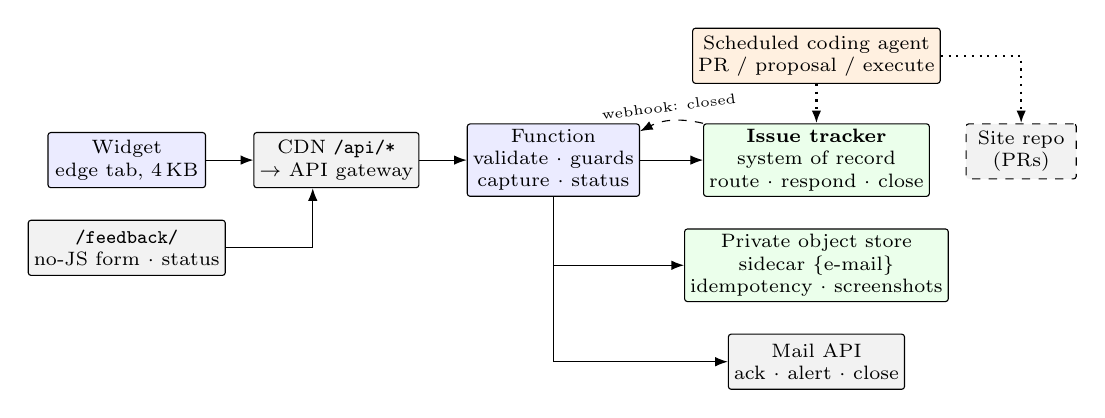
\begin{tikzpicture}[
  font=\scriptsize, node distance=4mm and 6mm,
  box/.style={draw, rounded corners=1pt, minimum height=7mm, minimum width=20mm, inner sep=2pt, align=center},
  ext/.style={box, fill=black!5}, ours/.style={box, fill=blue!8}, store/.style={box, fill=green!8}, agent/.style={box, fill=orange!12},
  arr/.style={-{Latex[length=1.6mm]}}, loop/.style={arr, dashed}, ag/.style={arr, dotted, thick}]
  \node[ours] (widget) {Widget\\edge tab, 4\,KB};
  \node[ext, below=of widget] (page) {\texttt{/feedback/}\\no-JS form $\cdot$ status};
  \node[ext, right=of widget] (cdn) {CDN \texttt{/api/*}\\$\to$ API gateway};
  \node[ours, right=of cdn] (fn) {Function\\validate $\cdot$ guards\\capture $\cdot$ status};
  \node[store, right=8mm of fn] (tracker) {\textbf{Issue tracker}\\system of record\\route $\cdot$ respond $\cdot$ close};
  \node[agent, above=5mm of tracker] (agentn) {Scheduled coding agent\\PR / proposal / execute};
  \node[store, below=of tracker] (s3) {Private object store\\sidecar \{e-mail\}\\idempotency $\cdot$ screenshots};
  \node[ext, below=of s3] (mail) {Mail API\\ack $\cdot$ alert $\cdot$ close};
  \node[ext, dashed, below=5mm of agentn, xshift=26mm, minimum width=14mm] (repo) {Site repo\\(PRs)};
  \draw[arr] (widget) -- (cdn); \draw[arr] (page) -| ($(cdn.south)+(-3mm,0)$); \draw[arr] (cdn) -- (fn);
  \draw[arr] (fn) -- (tracker); \draw[arr] (fn) |- (s3); \draw[arr] (fn) |- (mail);
  \draw[loop] (tracker.north west) to[bend right=20] node[above, font=\tiny, sloped]{webhook: closed} ($(fn.north east)+(0,-1mm)$);
  \draw[ag] (agentn) -- (tracker);
  \draw[ag] (agentn.east) -| (repo.north);
\end{tikzpicture}}
\caption{Reference architecture. Solid: capture path; dashed: loop closure; dotted: agentic Respond stage. Blue: built for \ffrs; green: stores (the tracker is the system of record); grey: existing platform services.}
\label{fig:arch}
\end{figure}

\subsection{Capture surface}
A framework-free widget (one script tag, configured by data attributes) renders an edge tab on every page. It offers ``request a feature'' and ``report a bug'', captures the page URL and---for bugs---a client-side screenshot, and takes an optional e-mail with an explicit consent checkbox. A plain HTML form at \texttt{/feedback/} is the no-JavaScript fallback and the landing page for status links.

\subsection{Tracker as system of record}
The function validates the submission, applies guards (honeypot, per-address rate limit, a bot check), stores the screenshot in a private object store, and creates the issue synchronously with labels \texttt{kind:*}, \texttt{severity:*} and a hidden marker carrying the reference id. Only then does it return \texttt{202 \{ref\}}. If the tracker is unavailable the caller receives an honest \texttt{502} and the widget retries with the same idempotency key---nothing is half-stored. Route therefore coincides with Capture; Respond and Close are read from the tracker itself (first human comment, close event, \texttt{outcome:*} labels or close reason).

\subsection{Sidecar for personal data}
The only personal datum, the requester's e-mail, never enters the public record. A per-item JSON object in a private object-store prefix holds \{e-mail, consent, screenshot key, ack sent, closing mail sent\}. Deleting that object forgets the person; screenshots and idempotency keys expire automatically.

\subsection{Loop closure}
A tracker webhook fires on close; the function derives the outcome (\texttt{outcome:*} label $\succ$ close reason $\succ$ kind default) and sends the closing note. Comments and close time need no webhook---the tracker already records them.

\subsection{Agentic Respond stage}
A scheduled cloud agent runs against the tracker. For each open item without a first response, it either opens a pull request on the target repository (code path) or posts a proposal comment (proposal path). Acceptance and confirmation are ordinary comments matching a small command grammar (\texttt{/accept}, \texttt{/confirm}, \texttt{/reject <reason>}) by the requester and by a maintainer respectively; the agent executes a proposal only after a maintainer's confirmation (a requester without a tracker account cannot accept; the maintainer then acts for both). In the reference deployment the agent is a hosted coding-agent routine that runs hourly with the site and tracker repositories checked out and the host's tracker tools available (Sec.~\ref{sec:impl}); any coding agent that can read the tracker, run the project's tests and open a pull request fits the role. Its instructions are a versioned prompt of about 700 words that fixes the selection rule (open items with a kind label and no prior response, oldest first, at most three per run), the two paths, the label protocol, a 15-minute budget with at most five minutes on test infrastructure, and the rules \emph{never push to main, never force-push, one branch per item, clean up temporary files}. ``Execute'' for a static site means a pull request (content or code) or a drafted reply; the agent has no other write path. Its tracker identity is the maintainer's, so agent comments carry a fixed marker and are excluded from the human metrics. A self-hosted CI-runner variant with the same protocol is kept as an alternative.
\subsection{Security and threat model}
An agent reading untrusted input from the public internet and executing code changes introduces the risk of indirect prompt injection. A malicious requester could embed instructions in the feedback description attempting to exfiltrate repository secrets or push harmful code. \ffrs{} mitigates this structurally: the agent runs in a heavily restricted sandbox with read-only access to the primary repository, and is only permitted to push branches to a constrained \texttt{ffrs/*} namespace. The environment contains no production secrets. Furthermore, the mandatory human-in-the-loop checkpoint ensures that even if an injection attack successfully commands the agent to generate a malicious payload, it cannot be merged into the mainline without maintainer review.


\subsection{Operability and audit trail}
Every layer is declared in version control and changed only through it: the site and widget are built from a repository, the function is a versioned bundle, the cloud resources are infrastructure-as-code, and the agent's protocol and prompt are files in the same repositories. Infrastructure changes go through \texttt{plan}/\texttt{apply} from a reviewed commit; content and code changes---including every change the agent proposes---arrive as pull requests. Consequently the audit trail for any question (\emph{who changed what, when, and why; which items the agent touched; what a reviewer approved}) is the commit and pull-request history plus the public tracker, with no separate audit store to maintain. Three switches make \ffrs{} detachable: a build-time flag (ships zero widget bytes), a runtime kill switch in the parameter store (\texttt{503} within a minute, no deploy), and an infrastructure flag that removes every resource; each is itself a committed change. Secrets are read at cold start from the parameter store and never appear in infrastructure state or in the repositories.

\section{Implementation}\label{sec:impl}
Table~\ref{tab:impl} summarises the reference implementation---one instantiation of the roles in Table~\ref{tab:roles}, chosen because the project already ran on that cloud and that code host. All artefacts are public; commit hashes pin the versions evaluated. Everything product-specific is confined to two adapters (tracker, object store), the mail sender, and the deployment module; the domain logic, guards, widget and metrics do not depend on the products named here.

\begin{table}[t]
\centering\footnotesize
\caption{Reference implementation at T0 (2026-09-23).}
\label{tab:impl}
\begin{tabular}{@{}l>{\raggedright\arraybackslash}p{5.4cm}@{}}
\toprule
API (\texttt{ffrs-api}) & Node~22 Lambda, TypeScript strict, Zod at every boundary; 26 files, $\approx$1{,}100 LOC, 44 tests (in-memory tracker/store twins, no network); 476\,KB bundle \\
Widget & 12.3\,KB (4.9\,KB gz), styles included; shadow DOM, no framework; screenshot library loaded on demand \\
Infrastructure & Terraform module, 23 resources (function and function URL, CDN distribution, asset and private buckets, mail identity, weekly rule) \\
Store & GitHub issue + one JSON sidecar per item; 0 tables; tenants in the parameter store \\
Agent & hosted coding-agent routine, hourly; $\approx$850-word versioned prompt (\texttt{agent/routine-prompt.md}) \\
Build effort & $\approx$1 working day across 8 phases (commit timeline in the repositories) \\
Run cost & within AWS free tier at the reference volume \todo{confirm after 4 weeks} \\
\bottomrule
\end{tabular}
\end{table}

\paragraph{Engineering standards} TypeScript strict with schema validation at every boundary; persistence behind two ports with in-memory twins so the test suite needs no network; structured logs keyed by the item's reference; formatting and validation before every infrastructure commit; small, single-purpose commits with imperative messages so the history reads as a change log. Infrastructure as code and GitOps are applied uniformly, making the audit trail in Sec.~\ref{sec:arch} complete rather than partial.

\paragraph{Embedding contract} A site adopts \ffrs{} with one tag:
\begin{lstlisting}
<script src="https://<service-host>/widget.js"
  data-site="example" data-turnstile="<sitekey>"
  data-screenshot="bug" defer></script>
\end{lstlisting}
and a tenant entry (tracker repository and token, allowed origins, optional secrets). Everything site-specific is an attribute or a tenant setting; nothing is deployed per site.

\paragraph{Research export} Each week the function files a metrics report in every tenant's tracker and, for tenants that opted in, writes one item-level row per item filed since T0 to the private store: a site pseudonym, kind, severity, outcome, agent path and the stage timestamps---never text, contact or links. The S2 figures in Sec.~\ref{sec:eval} are computed from these rows.

\paragraph{Reproducing the metrics} \texttt{npm run metrics} and \texttt{npm run export} in \texttt{ffrs-api} read a tracker and emit per-week metrics and anonymised per-item rows (no body, e-mail or screenshot) for items filed since T0. The CSVs used in Sec.~\ref{sec:eval} are committed under \texttt{data/} in the paper repository.

\section{Evaluation}\label{sec:eval}
\subsection{Setting}
Two sites are studied, both served by the one deployment described in Secs.~\ref{sec:arch}--\ref{sec:impl} from T0, 23~September~2026, 18:00~CEST; items from earlier pilots and from the acceptance checks before T0 are excluded. \textbf{S1} is the reference site, scaledaiops.org; its Respond stage is the scheduled agent, and every item, comment, label and pull request is public. \textbf{S2} is an anonymous B2B quick-commerce platform supplying restaurants, in its pre-launch phase, that embeds the same widget and routes items to its own private tracker, where its maintainers respond manually. It contributes the anonymised research rows of Sec.~\ref{sec:impl} only. Because capture, tracker and metric pipeline are identical on both sites, S2 is a comparison point for the Respond stage itself: agentic versus human first response.
\subsection{Protocol}
The protocol was fixed in the project's case-study document before data collection: a 12-week window from T0 (to 16~December~2026) with an interim read-out at week~4 (21~October~2026); per-kind, per-ISO-week metrics as defined in Sec.~\ref{sec:model}; targets stated in advance---TTFR under two hours (the agent's schedule), TTHR under 72~h at the median, TTC for bugs under 30 days at the median, closing notification for 100\,\% of consented closed items---and signal ratio and agent share reported without a target. The source of truth is, for S1, the public tracker read by the published \texttt{metrics}/\texttt{export} commands and, for S2, its weekly research rows; the resulting CSVs are committed with their export date. Items filed by the maintainer to test the system are labelled \texttt{spam} in the tracker and excluded.
\subsection{Results at week 4}
Table~\ref{tab:metrics} will report the interim metrics for both sites against the pre-registered targets; the values are filled from the committed week-4 export (\todo{2026-10-21}) and are deliberately blank until then. Operating cost (RQ1) will be reported from the actual cloud bill for the shared deployment; the agent runs within a subscription and has no per-item API charge.

\begin{table}[htbp]
\centering\footnotesize
\caption{Interim evaluation metrics (week 4). Targets are pre-registered; S2 responds without the agent.}
\label{tab:metrics}
\begin{tabular}{@{}l@{\hspace{0.75em}}l@{\hspace{0.75em}}r@{\hspace{0.75em}}r@{\hspace{0.75em}}r@{}}
\toprule
Metric & Target & S1 (bugs) & S1 (features) & S2 (all) \\
\midrule
$n$ (signal) & --- & \todo{} & \todo{} & \todo{} \\
TTFR (p50 / p90) & $<2$\,h & \todo{} & \todo{} & \todo{} \\
TTHR (p50) & $<72$\,h & \todo{} & \todo{} & \todo{} \\
TTC (p50) & $<30$\,d (bugs) & \todo{} & \todo{} & \todo{} \\
Loop closure & --- & \todo{} & \todo{} & \todo{} \\
Consented notification & 100\,\% & \todo{} & \todo{} & \todo{} \\
Signal ratio & --- & \todo{} & \todo{} & \todo{} \\
Agent share & --- & \todo{} & \todo{} & n/a \\
\bottomrule
\end{tabular}
\end{table}

\subsection{Ablation (RQ3)}
The dependency-minimal architecture is the result of removing components from an earlier design; we argue for the load-bearing role of what remains:
\begin{itemize}
    \item \textbf{Issue tracker vs.\ dedicated database:} the initial design had a relational store and an outbox. Removing them simplified the system and moved durability to the tracker; the trade-off is synchronous coupling---if the tracker is down, capture fails with an explicit \texttt{502} and the client retries safely with its idempotency key.
    \item \textbf{Sidecar vs.\ public personal data:} the private sidecar isolates e-mail addresses and screenshots; without it a public tracker could not be the system of record.
    \item \textbf{Bot check and honeypot:} protect the signal ratio by rejecting automated submissions before an issue is created; the counts of rejected and spam-labelled items are reported at week~4.
\end{itemize}

\section{Discussion}\label{sec:discussion}
\subsection{When a minimal, agentic loop is sufficient}
The reference deployment suggests three conditions under which \ffrs{} as described is enough. First, the project already lives in one tracker: routing is then a label, respond and close are events the tracker records anyway, and there is nothing to synchronise. Second, most items are small: content corrections, wording, missing links, configuration---exactly the class an agent resolves end to end with a reviewable pull request. Third, maintainer attention is the binding constraint, not code-review capacity: the agent shifts effort from \emph{producing} a first response to \emph{judging} one, and judging a two-line diff takes a minute. Under these conditions the human role reduces to merge, accept and confirm, and the loop closes without anyone owning a queue.

\subsection{Where it breaks}
The same conditions delimit the design. Items that need a decision the project has not made (scope, policy, roadmap) go down the proposal path and wait for a human exactly as before; the agent makes the waiting \emph{visible} (a proposal with a timestamp) but not shorter. Requesters without a tracker account cannot accept a proposal, so the reviewer acts for both---acceptable for a small site, not for a product with many stakeholders. A project with several teams needs routing beyond a label. And an agent that opens pull requests is only as safe as the review culture around it: \ffrs{} makes the review checkpoint structural, but a maintainer who merges without reading has removed it.

\subsection{Removing the database was the right cut}
The first design had a relational database, an outbox and a metrics view. Replacing them with the tracker as system of record removed one external service, one secret, one schedule and roughly a third of the code, and it made every metric recomputable by anyone with read access. What it cost was buffering: capture is now synchronous with the tracker, and an outage yields an honest \texttt{502} and a client-side retry rather than a queued item. For a small project this is the better trade---the tracker's availability is already the project's availability---and it keeps the whole system explainable in one diagram.

\subsection{What the build taught us about agents in the loop}
Two production-only findings shaped the agent's operating envelope. The first agent run produced a correct fix within eight minutes and then failed on permissions: it could read the organisation's repositories but not write, and it reported this precisely instead of retrying. The second run succeeded but spent most of its time on test infrastructure that did not match the sandbox. Both point to the same lesson: an agentic Respond stage needs a budget and an escape hatch (``state what you could not run and ship the pull request'') more than it needs cleverness, and the surrounding tooling---installable browsers, hermetic tests---matters as much as the prompt. Once both were in place, a real request was resolved by an agent pull request and a one-minute human review.

\subsection{Cost}
At the reference site's volume the whole system runs within a cloud free tier and the agent within a subscription; the marginal cost of an item is the reviewer's minute. We report actual figures in Sec.~\ref{sec:eval} once the measurement window closes.

\section{Threats to Validity}\label{sec:threats}
\paragraph{Internal validity}
The maintainer of the reference site is also the author of this paper and the reviewer in the loop; time to first human decision (TTHR) and time to close are therefore likely flattering relative to a project whose maintainers did not build the system. We mitigate by pre-registering targets and the measurement protocol before data collection, by reporting per-item timelines rather than only aggregates, and by excluding items we filed ourselves to test the system (labelled \texttt{spam} in the public tracker, visible to anyone). The agent's own responses are posted under the maintainer's tracker identity; we distinguish them by a fixed marker so that TTHR counts only human comments, and we report TTFR (agent or human) separately.

\paragraph{External validity}
The evaluation covers one small, niche, non-commercial site plus aggregate figures from one independent commercial deployment; feedback volume is low, so all rates are reported with $n$ and no inferential statistics are claimed. The reference implementation targets one tracker and one cloud provider; the model depends on neither (Table~\ref{tab:roles}), and the tracker sits behind a two-method port, but a second adapter has not been built and exercised. Results for larger teams, higher volumes or regulated domains are out of scope.

\paragraph{Construct validity}
``Respond'' is operationalised as the first comment or pull request on the item, which may be a question or an incorrect attempt rather than an answer; ``close'' is the tracker's close event with an inferred outcome, which measures that a decision was recorded, not that the requester was satisfied. Loop closure is a system property (a closing notification was sent) and not a satisfaction measure. Signal ratio depends on maintainers labelling spam consistently. Agent share counts merged agent pull requests and executed proposals; it says nothing about the effort a reviewer spent correcting them, which we report qualitatively only.

\paragraph{Reliability}
All metrics are recomputable by anyone with read access to the public tracker using the published tooling; the CSV exports used in this paper are committed with their export dates. The dependence on the tracker cuts both ways: an outage or a change in the tracker's API affects capture (an explicit \texttt{502} and client retry) and measurement, and comment timestamps are the tracker's, not ours.

\paragraph{Ethical considerations}
Personal data is limited to an optional e-mail stored with explicit consent, apart from the public record, and deletable; screenshots may capture on-screen content and are therefore private and expiring; the agent never acts on production without a human decision, and every action it takes is visible in the public tracker.

\section{Related Work}
\paragraph{Flow metrics and developer productivity}
\ffrs{}'s metrics are descendants of established flow vocabularies. The DevOps programme summarised in \emph{Accelerate}~\cite{forsgren2018accelerate} and later expanded in the SPACE framework~\cite{forsgren2021space} popularised outcome metrics---lead time for changes, deployment frequency---chosen because they can be measured mechanically. ITIL~4~\cite{axelos2019itil} frames request handling as a sequence of acknowledgement, routing, and resolution targets. \ffrs{} borrows the shape of both but reduces the scope to what one tracker can carry: no service desk, no separate measurement system. Where DORA measures the path from commit to production, \ffrs{} measures the path from stakeholder to outcome; where ITIL assumes a staffed queue, \ffrs{} assumes an agent produces the first response.

\paragraph{Issue handling and maintainer fatigue}
Large-scale mining studies established both the centrality and fragility of issue trackers. Bissyand\'e et al.~\cite{bissyande2013gotissues} found that responsiveness varies widely, while Kalliamvakou et al.~\cite{kalliamvakou2014promises} catalogued the pitfalls of interpreting tracker data. Unmanaged queues are among the reasons open source projects fail~\cite{coelho2017why}. \ffrs{} takes these findings as motivation: the tracker is where decisions are made, so \ffrs{} keeps it as the system of record and instruments it, assigning the first response to an agent to mitigate fatigue.

\paragraph{Autonomous issue resolution}
SWE-bench~\cite{jimenez2024swebench} made ``resolve a real GitHub issue with a pull request'' a benchmark task. SWE-agent~\cite{yang2024sweagent}, Agentless~\cite{xia2024agentless}, ChatDev~\cite{qian2023chatdev}, and RepairAgent~\cite{bouzenia2024repairagent} have demonstrated that language models with purpose-built interfaces can resolve issues unattended at meaningful rates. \ffrs{} does not advance agent capability. Instead, it positions the agent as the \emph{default} owner of the Respond stage in a feedback loop, bounded by human checkpoints (merge for code; requester acceptance and reviewer confirmation for proposals), and it measures the result with the same timestamps as human-only handling. To our knowledge the combination---a feedback pipeline model, an agentic first response, and metrics recomputable from the public tracker---has not been described as a unit.

\paragraph{In-product feedback tooling and mining}
Extracting features and bugs from user feedback is a rich area of research, with tools like SAFE~\cite{johann2017safe} and various machine learning classifiers for app reviews~\cite{panichella2015how, guzman2014how}. While commercial widgets (e.g., Sentry, Intercom) provide the capture surface, they rely on vendor-hosted storage. \ffrs{} sits between these: an anonymous, account-free capture surface that funnels directly into the public tracker, avoiding proprietary databases while keeping personal data in a private sidecar.

\section{Conclusion}
Feedback loops in small software projects fail in the interval between ``raised'' and ``acted on'', and they fail invisibly because that interval is unmeasured. \ffrs{} makes the interval visible and hands its first half to an agent. The model is deliberately small: five stages, each a timestamp recorded by the system that owns it; four metrics that follow from those timestamps; and one structural rule---the Respond stage is performed by a scheduled agent, bounded by human checkpoints (merge for code; accept-and-confirm for proposals). The reference implementation adds no system of record beyond the tracker a project already has: a 4\,KB widget, one serverless function, a private sidecar for the only personal datum, and a scheduled cloud coding agent. It was built in about a working day, is removable through a three-layer toggle, and has run in production on scaledaiops.org since 18~August~2026, where a real request has already been captured, resolved by an agent-authored pull request, reviewed in a minute, merged and closed.

We claim no more than the evidence supports: that a minimal, agentic feedback loop is \emph{sufficient} for a small project under conditions we make explicit, and that its behaviour can be measured by anyone from public data. Future work is measurement over a longer window and more sites, a second tracker and runtime (for example a Jira-backed, container-hosted instance) to demonstrate the substitutability claimed in Table~\ref{tab:roles}, closure notifications that do not depend on e-mail, and a study of reviewer effort on agent-authored changes---the quantity that ultimately decides whether the human checkpoint stays a checkpoint or becomes the new bottleneck.


\section*{Acknowledgements}
The FFRS concept and its design are the author's. Parts of the implementation and of this manuscript were produced with an AI coding assistant under the author's direction; all claims and data were verified by the author. The ScaledAIOps community hosts the reference deployment.

\section*{Availability}
Code (MIT): \href{https://github.com/Scaled-AIOps/ffrs-api}{Scaled-AIOps/ffrs-api}; widget (CC~BY-SA~4.0): \href{https://github.com/Scaled-AIOps/scaledaiops.org}{Scaled-AIOps/scaledaiops.org}; infrastructure: \href{https://github.com/Scaled-AIOps/aiops-tf-infra}{Scaled-AIOps/aiops-tf-infra}. Feedback tracker (public data source): \href{https://github.com/Scaled-AIOps/feedback}{Scaled-AIOps/feedback}. Metrics are reproducible with \texttt{npm run metrics} against that repository.

\bibliographystyle{IEEEtran}
\bibliography{refs}
\end{document}
